\documentclass[10pt]{article}
\usepackage{../../local}

\usepackage{mathbbol}
\DeclareSymbolFontAlphabet{\mathbbold}{bbold}						% Blackboard Bold Numbers with \mathbbold


\newcommand{\classcode}{Physics W89}
\newcommand{\classname}{Mathematical Methods in Physics}
\renewcommand{\maketitle}{%
\hrule height4pt
\large{Eric Du \hfill \classcode}
\newline
\large{HW Final} \Large{\hfill \classname \hfill} \large{\today}
\hrule height4pt \vskip .7em
\normalsize
}
\linespread{1.1}
\begin{document}
	\maketitle
	\section*{Problem 1}
	\begin{enumerate}[label=\alph*)]
		\item Find the Eigenvalues of $A$. Verify that $\vec v_1$ is indeed an eigenvector and find 
			its eigenvalue. Pick \textit{one} of the remaining two eigenvalues and find the 
			eigenvector (you don't need to normalize)

			\begin{solution}
				To show that $\vec v_1$ is an eigenvector, we can just compute $A \vec v_1$:
				\[
					A \vec v_1 = \begin{pmatrix} 1 & 0 & 2i \\ 0 & 3 &0\\2i & 0 & -2 \end{pmatrix} 
					\begin{pmatrix} -2i\\0\\1 \end{pmatrix} = 
					\begin{pmatrix} -2i - 2i\\0 \\ -4i^2 - 2 \end{pmatrix} 
					= \begin{pmatrix} -4i\\0\\2 \end{pmatrix} = 2\begin{pmatrix} -2i \\0 \\ 1 \end{pmatrix} 
				\] 
				so we see that we get back $\vec v_1$, meaning it is an eigenvector, and its 
				associated eignenvalue is 2. 


				To find the other eigenvalues, we find the characteristic polynomial using $\det(A - \lambda 
				\mathbbold 1) = 0$:
				\begin{align*}
					0&=\begin{vmatrix} 1 - \lambda& 0 & 2i\\0 & 3-\lambda & 0\\2i & 0 & -2 - \lambda\end{vmatrix}
					\\
					 &= (1 - \lambda) (3 - \lambda)(-2 - \lambda) + (-2i)(-(3 - \lambda) (2i))\\
					 &= -(1 - \lambda)(6 + \lambda - \lambda^2) - 12 + 4\lambda\\
					 &= -6 - \lambda +  \lambda^2 + 6\lambda + \lambda^2 - \lambda^3 - 12 + 4\lambda \\
					 &= -\lambda^3 + 2\lambda^2 + 9\lambda - 18
				\end{align*} 
				We can use a root finder here, which will give us eigenvalues of $\lambda = -3, 3, 2$. Since
				$\lambda = 2$ is given by $\vec v_1$, we'll do $\lambda = 3$. To find the eigenvector, 
				we now solve the equation $\det(A - 3 \mathbbold 1) = \vec 0$. This can be done by 
				augmenting our matrix with zeroes on the right column: 
				\[
					\tilde A = \begin{pmatrix} -2 & 0 & -2i&0\\0&0&0&0\\2i&0&-5&0 \end{pmatrix} 
				\] 
				Now we can begin the process of row reduction. First, swap rows 2 and 3, and also divide 
				row 1 by 2:
				\[
					\begin{pmatrix} 1&0&i&0\\2i&0&-5&0\\0&0&0&0 \end{pmatrix} 
				\] 
				Now subtract row 2 by $2i$ times row 1, ($R_2 - 2iR_1$):
				\[
					\begin{pmatrix} 1&0&i&0\\0&0&-3&0\\0&0&0&0 \end{pmatrix} 
				\] 
				At this point, we can divide row 2 by 2, thereby making it a pivot, then use the pivot 
				to kill the third entry in the first row. Doing so, we get:
				\[
					\begin{pmatrix} 1&0&0&0\\0&0&1&0\\0&0&0&0 \end{pmatrix} 
				\] 
				Using the vector $\begin{pmatrix} a\\b\\c \end{pmatrix}$, this gives the equations
				$a = 0$ and $c = 0$, but there's no condition on $b$. Thus, any vector of the form 
				$\vec v = \begin{pmatrix} 0 \\b\\0 \end{pmatrix}$ would be an eigenvector. In its simplest form, 
				$b = 1$, so our eigenvector is 
				\[
				\vec v_2 = \begin{pmatrix} 0\\1\\0 \end{pmatrix} 
				\] 
				Also, as per the exam policy, I admit that I did use Mathematica to verify that this is indeed
				the correct eigenvector.
			\end{solution}
		\item Find the rotation matrix $R_{[e]}(\theta)$. 

			\begin{solution}
				We'll first find $R_{[f]}$, since the matrix $L_{[f]}$ is diagonal in this basis, so it allows
				for easy application of the exponential. Recall the convenient relation for diagonal matrices:
				\[
					f(D) = \begin{pmatrix} f(d_{11}) & \dots &0 \\
					\vdots & \ddots & \vdots \\
					0& \dots & f(d_{nn})\end{pmatrix} 
				\] 
				provided that $f$ is a Taylor-expandable function. Since $e^x$ is such a function, we can 
				apply this result here to make our lives very easy:
				\[
					R_{[f]}= e^{\theta L_{[f]}} = \exp{\begin{pmatrix} i \theta & 0\\0 & -i\theta \end{pmatrix} }
					= \begin{pmatrix} e^{i \theta} & 0 \\ 0 & e^{-i \theta}\end{pmatrix} 
				\] 
				Now we have to find $R_{[e]}$, which can be found by performing a change of basis, $R_{[e]} = 
				C^\dagger R_{[f]} C$. Therefore:
				\begin{align*}
					R_{[e]}(\theta) &= \frac{1}{\sqrt{2} }\begin{pmatrix} 1&1\\-i&i \end{pmatrix} \begin{pmatrix} e^{i \theta} & 0 \\ 0 & e^{- i \theta} \end{pmatrix} \frac{1}{\sqrt{2} }\begin{pmatrix} 1 & i\\ 1& -i \end{pmatrix} \\
									&= \frac{1}{2}\begin{pmatrix} 1&1\\-i&i \end{pmatrix} \begin{pmatrix} e^{i \theta}&ie^{i \theta} \\ e^{-i\theta} & -ie^{- i \theta}  \end{pmatrix}  \\
									&= \frac{1}{2}\begin{pmatrix} e^{i \theta} + e^{-i \theta} & i(e^{i \theta} - e^{- i \theta}\\ i(e^{-i \theta} - e^{i \theta}) & e^{i \theta} + e^{- i \theta} \end{pmatrix}  
				\end{align*}
				Here's where we remember our good old formulas for sine and cosine:
				\[
					\sin(\theta) = \frac{e^{i \theta} - e^{- i \theta}}{2i} \ \ 
					\cos(\theta) = \frac{e^{i \theta} + e^{- i \theta}}{2}
				\] 
				Therefore, this simplifies to:
				\[
					R_{[e]}(\theta) = \frac{1}{2}\begin{pmatrix} 2 \cos \theta & -2 \sin \theta\\
						2\sin \theta & 2\cos \theta \end{pmatrix} = \begin{pmatrix} \cos \theta&-\sin \theta\\
					\sin \theta & \cos \theta\end{pmatrix} 
				\] 
				Which just so happens to be our familiar formula for 2D rotation.
			\end{solution}
		\item Solve Eq. 1 with the initial condition $h(0) = h_0$ to find $h(t)$. For what range of $t$ 
			does our solution make physical sense?

			\begin{solution}
				First, divide both sides by $B$: 
				\[
					\dv{h}{t} = -\frac{\mu A}{B} \sqrt{2g} \cdot \sqrt{h} 
				\] 
				Let's let $-k = - \frac{\mu A}{B}\sqrt{2g}$ to clear up the clutter of constants. This now 
				means we have the differential equation:
				\[
					\dv{h}{t} = -k \sqrt{h} 
				\] 
				This differential equation can be solved by separation of variables:
				\begin{align*}
					\frac{\mathrm dh}{\sqrt{h} } &= -k \mathrm dt\\
					\int \frac{\mathrm dh}{\sqrt{h}} &= -\int k \ \mathrm dt \\
					2\sqrt{h(t)} &= -kt + C
				\end{align*}
				Solving for $h(t)$, we get:
				\[
				h(t) = \left( -\frac{kt}{2} + C \right)^2
				\] 
				The constant $C$ can be solved using the initial condition $h(0) = h_0$:
				\[
				h_0 = C^2 \implies C = \sqrt{h_0} 
				\] 
				We reject the negative solution $C = -\sqrt{h_0}$ since having a negative height makes no sense.
				Therefore, our full solution is:
				\[
				h(t) = \left( -\frac{\mu A t}{2B}\sqrt{2g}  + \sqrt{h_0} \right)^2
				\] 
				Further, this equation only makes sense starting from $t = 0$ until the moment when 
				$h(t)$ reaches zero (since our tank can't drain further). The root occurs at:
				\[
				-\frac{\mu A t}{2B}\sqrt{2g}  + \sqrt{h_0} = 0 \implies t = \frac{2B \sqrt{h_0}}{\mu A \sqrt{2g} }
				\] 
				Therefore, our equation only makes sense from $t =0$ to $t = \frac{2B}{\mu A}\sqrt{\frac{h_0}{2g}} $. 
				In reality, after this time, the equation $h(t)$ begins to rise (since it's quadratic), 
				which again isn't physical in our context since this would imply that the water height 
				is increasing despite not adding any water into the bucket. 
			\end{solution}
		\item First, starting from an ansatz, find a pair of linearly independent solutions to the homogeneous
			version of Eq. 1. Then find a particular solution to this inhomogeneous ODE. 
			
			\begin{solution}
				The homogeneous equation is:
				\[
				\ddot y + 2b\dot y + \omega_0y = 0
				\] 
				This differential equation can be solved using the ansatz \footnote{
					Technically speaking, I think there should be an $Ae^{\lambda t}$ to account for 
				initial conditions, but this constant can be handled also by the linear combination, which 
			is also a solution to the homogeneous ODE.} of 
				$y = e^{\lambda t}$.  Computing
				derivatives:
				\begin{align*}
					\dot y &= \lambda e^{\lambda t}\\
					\ddot y &= \lambda^2 e^{\lambda t}
				\end{align*}
				Plugging this into the homogeneous ODE:
				\[
					\lambda^2 e^{\lambda t} + 2b \lambda e^{\lambda t} + \omega_0^2 e^{\lambda t} = 0 \implies
					\lambda^2 + 2b \lambda + \omega_0^2 = 0
				\] 
				Therefore, we can use the quadratic equation, to find the solutions:
				\begin{align*}
					\lambda_{\pm} &= \frac{-2b \pm \sqrt{(4b)^2 - 4 \omega_0^2} }{2} \\
					&= -b \pm \sqrt{b^2 - \omega_0^2}  
				\end{align*}
				Since $b < \omega_0$, this quantity is complex, and using $\widetilde \omega$ from the problem
				statement, we can write this as:
				\[
				\lambda_\pm = -b \pm i \widetilde \omega
				\] 
				We also confirm that these two solutions are linearly independent, since they are different
				exponentials (we proved this in homework). To find the particular solution, we can use 
				variation of parameters, since our inhomogeneity isn't an element of our table of 
				guesses. For the sake of clarity, I will use $\lambda_1 = -b + i \widetilde \omega$ and
				$\lambda_2 = -b - i \widetilde \omega$
				to refer to the exponents of the two homogeneous solutions. Our general solution 
				with the variation of parameters approach is to have solution of the form 
				$y(t) = c_1(t)y_{h 1}(t) + c_2(t) y_{h 2}(t)$. Before we get to calculating $c_1$ and $c_2$, 
				let's first find the Wronskian, which will be useful later:
				\[
					W(t) = \begin{vmatrix} e^{\lambda_1 t} & e^{\lambda_2 t}\\ \lambda_1e^{\lambda_1 t} & 
					\lambda_2e^{\lambda_2 t} \end{vmatrix} = \lambda_2e^{(\lambda_1 + \lambda_2) t} -
					\lambda_1e^{(\lambda_1 + \lambda_2)t} = e^{(\lambda_1 + \lambda_2) t}(\lambda_2 - \lambda_1)
				\] 
				With that out of the way, we are ready to construct the particular solution. From lecture, we 
				know that for an ODE with two homogeneous solutions, we have the set of equations (this 
				form comes directly as a result of Cramer's rule):
				\[
					\dot c_1(t) = \frac{\det\begin{pmatrix} 0 & y_{h 2}(t)\\ r(t) & \dot y_{h 2}(t)\end{pmatrix}}{W(t)} \ \ 
					\dot c_2(t) = \frac{\det\begin{pmatrix} y_{h 1}(t) & 0 \\ \dot y_{h 1}(t) & r(t) \end{pmatrix} }{W(t)} 
				\] 
				where $y_{h 1}(t)$ and $y_{h 2}(t)$ refer to the homogeneous solutions, and $r(t)$ is our 
				inhomogeneity. Thus, plugging everything in, we get:
				\[
					\dot c_1(t) = \frac{\det\begin{pmatrix} 0 & e^{\lambda_2 t}\\ A\delta(t - t_0) & \lambda_2e^{\lambda_2t} \end{pmatrix}}{W(t)} = -\frac{Ae^{\lambda_2 t} \delta(t - t_0)}{e^{(\lambda_2 + \lambda_1) t}(\lambda_2 - \lambda_1)}
				\] 
				Likewise for $c_2(t)$, skipping the algebra here: 
				\[
					\dot c_2(t) = \frac{Ae^{\lambda_1 t}\delta(t - t_0)}{(\lambda_2 - \lambda_1) e^{(\lambda_1 + \lambda_2) t}}
				\] 
				Then to find $c_1(t)$ and $c_2(t)$, we integrate both of these from $0$ to $t$ (this also 
				comes from the lecture notes):
				\begin{align*}
					c_1(t) &= \int_0^t -\frac{Ae^{\lambda_2 t} \delta(t - t_0)}{e^{(\lambda_2 + \lambda_1) t}(\lambda_2 - \lambda_1)} dt \\
					c_2(t) &= \int_0^t \frac{Ae^{\lambda_1 t}\delta(t - t_0)}{(\lambda_2 - \lambda_1) e^{(\lambda_1 + \lambda_2) t}} dt 
				\end{align*}
				Now $t_0$ is some positive value. Recall that for a Dirac delta, 
				\[
				\int_a^b f(u)\delta(u - u_0) = \begin{cases}
					f(u_0) & a < u_0 < b\\
					0 & \text{else}
				\end{cases}
				\] 
				So in order for our integral to be nonzero, we require that $t > t_0$. When $t < t_0$, then
				we have $c_1(t) = c_2(t) = 0$. Therefore, we now have our solutions $c_1(t)$ and $c_2(t)$:
				\begin{align*}
					c_1(t) &= \begin{cases}
						0 & 0 \le t < t_0\\
						-\frac{Ae^{\lambda_2 t_0}}{(\lambda_2 - \lambda_1)e^{(\lambda_1 + \lambda_2) t_0}} & t > t_0
					\end{cases}\\
						c_2(t) &= \begin{cases}
							0 & 0 \le t < t_0\\
							\frac{Ae^{\lambda_1 t_0}}{(\lambda_2 - \lambda_1)e^{(\lambda_1 + \lambda_2) t_0}}	&t > t_0
						\end{cases}
				\end{align*}
				We can now plug back in the values $\lambda_1 = -b + i \sqrt{\omega_0^2 - b^2}$ and 
				$\lambda_2 = -b - i \widetilde \omega$. First, we can compute their sum and difference:
				\begin{align*}
					\lambda_2 - \lambda_1 &= - b - i \widetilde \omega - (-b + i \widetilde \omega) = 
					-2i \widetilde  \omega\\
					\lambda_2 + \lambda_1 &= -b - i \widetilde \omega + (-b + i \widetilde \omega) = -2b
			\end{align*} 
				Therefore, our $c_1(t)$ and $c_2(t)$ simplify to:
				\begin{align*}
					c_1(t) &= \begin{cases}
						0 & 0 \le t < t_0\\
						\dfrac{Ae^{(-b - i \widetilde \omega)t_0}}{2i \widetilde \omega e^{-2b t_0}} & t > t_0
					\end{cases}\\
						c_2(t) &= \begin{cases}
							0 & 0 \le t < t_0\\
							-\dfrac{Ae^{(-b + i \widetilde \omega) t_0}}{2i \widetilde \omega e^{-2b t_0}}	&t > t_0
						\end{cases}
				\end{align*}
				Therefore, our particular solution is of the form $y(t) = c_1(t)e^{(-b + i \widetilde \omega) t} + c_2(t)e^{-(b + i\widetilde \omega)t}$ where $c_1(t)$ and $c_2(t)$ are defined piecewise above. 
			\end{solution}
		\item Plug the power series ansatz of Frobenius, $y(x) = \sum_{m = 0} a_m x^{m + r}$, into this 
			ODE. Find the indical equation to determine $r$. Find the recursion relation from the coefficient 
			of the $x^{r + m}$ term ($m \ge 0$). Finally, find the solution for $n = 2$. 
			
			\begin{solution}
				First, we'll take derivatives of the ansatz:
				\begin{align*}
					y'(x) &= \sum_{m = 0}a_m (r+m)x^{r+m-1}\\
					y''(x) &= \sum_{m = 0}a_m (r+m)(r+m-1)x^{r + m-2} 
				\end{align*}	
				Therefore, our differential equation is: 
				\begin{multline*} 
					x \sum_{m = 0} a_m(r+m)(r+m-1)x^{r + m-2} + (1-x)\sum_{m =0}a_m (r+m)x^{r+m-1} + n\sum_{m = 0} a_m x^{r+m} = 0
				\end{multline*}
				Expanding out the $1-x$ term, we get:
				\begin{multline}\label{DE}
					\sum_{m = 0}a_m (r+m)(r+m-1)x^{r+m-1} + \sum_{m=0}a_m (r+m)x^{r+m-1}\\ - \sum_{m=0}a_m(r+m)x^{r+m} + n\sum_{m =0} a_m x^{r+m} = 0	
				\end{multline}
				To find the indical equation, we substitute in $m =0$ to get:
				\[
					a_0r(r-1) x^{r-1} + a_0 rx^{r -1} - a_0r x^{r} + na_0x^r = 0
				\] 
				We look specifically in front of the $x^{r-1}$ term, which gives us the equation:
				\[
				a_0r(r-1) + a_0r = 0 \implies r^2 = 0 \implies r = 0
				\] 
				Now to find the recursion relation, we have to shift the first two terms in equation \ref{DE} 
				over by 1 so that the exponents match up (while simultaneously letting $a_{-1} = 0$). At this
				point we can also substitute in $r=0$, meaning that we are looking at the coefficient of 
				the $x^m$ term now:
				\[
					\sum_{m = -1} a_{m+1}(m+1) m x^m + \sum_{m = -1} a_{m+1} (m+1)x^m - \sum_{m = 0}a_m mx^{m} + 
					n \sum_{m =0} a_m x^m = 0
				\]
				We can now throw this under one large summation:
				\[
					\sum_{m = -1} \left[a_{m+1}(m+1) m + a_{m+1} (m+1) - a_m m + n a_m \right] x^m = 0
				\] 
				The coefficient must be zero, so therefore we get the equation:
				\[
					\left[m(m+1) + (m+1) \right]a_{m+1} - \left[m- n\right]a_m= 0
				\] 
				Now solving for $a_{m+1}$:
				\[
					a_{m +1} = \frac{m - n}{m(m+1) + m+1} a_m = \frac{m-n}{(m+1)^2}a_m 
				\] 
				For $n=2$, the solution becomes: 
				\[
					a_{m+1} = \frac{m-2}{(m+1)^2}a_m	
				\] 
				We'll express the solution in terms of $a_0$. For $a_1$, we plug in $m=0$:
				\[
					a_1 = -\frac{2}{1} = -2a_0
				\] 
				Then for $a_2$, we plug in $m=1$:
				\[
				a_2 = -\frac{1}{2^2}= -\frac{1}{4}a_1 = \frac{1}{2}a_0
				\] 
				Then for $a_3$, we plug in $n = 2$, but we find that $a_3 = 0 a_2 = 0$. Since all 
				subsequent terms depend on $a_3$ recursively, we conclude that the sequence terminates. 
				Therefore, our polynomial is:
				\[
				y(x) = \frac{1}{2}a_0 x^2 - 2a_0 x + a_0
				\] 
			\end{solution}
	\item Find the exponential Fourier coefficients $c_n$ of this function.

		\begin{solution}
			The coefficients are calculated using the formula:
			\[
				c_n = \frac{1}{T}\int_{t_0}^{t_0 + T} e^{- in \omega_0 t} f(t) dt
			\] 
			We can choose $t_0 = 0$, giving us:
			\[
				c_n = \frac{1}{T}\int_0^T e^{-in \omega_0 t} A_0e^{-\alpha(t - mT)} dt = \frac{A_0}{T}
				\int_0^T e^{-(in \omega_0 + \alpha)t + \alpha mT} dt = \frac{A_0}{T} e^{\alpha mT}
				\int_0^T e^{-(in \omega_0 + \alpha) t} dt
			\] 
			This integral evaluates to:
			\begin{align*}
				c_n &= \frac{A_0}{T} e^{\alpha mT} \cdot \frac{1}{-(in \omega_0 + \alpha)}\left[ e^{-(in \omega_0 + \alpha) t}
				\right]_0^T\\
					&= \frac{A_0e^{\alpha mT}}{T(in \omega_0 + \alpha)}\left[1 - e^{-(in \omega_0 + \alpha)T}\right]\\
					&= -\frac{A_0e^{\alpha mT}}{T(in \omega_0 + \alpha)}\left[e^{-(in \omega_0 + \alpha)T} - 1\right]
			\end{align*}
			I don't see any real point in making the substitution $\omega_0 = \frac{2\pi}{T}$ since it 
			doesn't really lead to any meaningful simplifications, so this is my final answer. 
		\end{solution}
	\item Find the convolution $\Lambda_a(x) \equiv (\Pi_a \ast \Pi_a)(x)$ of the rectangular function
		with itself. Then find $\lambda_a(k)$, the Fourier transform of $\Lambda_a(x)$. 

		\begin{solution}
			The convolution of two functions is given as:
			\[
				(f \ast g)(x) = \int_{-\infty}^\infty f(s) g(x - s) ds
			\] 
			Substituting in the rectangular function, we have:
			\[
				(\Pi_a \ast \Pi_a)(x) = \int_{-\infty}^\infty \Pi_a(s) \Pi_a(x - s) ds
			\] 
			First thing to note is that this integral is only nonzero when $|s| < \frac{a}{2}$, since we
			need $\Pi_a(s)$ to be nonzero. This means we can change our integral bounds to:
			\[
				\Lambda_a(x) = \int_{-\frac{a}{2}}^{\frac{a}{2}} \Pi_a(x - s) ds
			\] 
			Now look at this visual diagram:
			\begin{center}
				\begin{tikzpicture}
					\draw (-2, 0) -- (2, 0);
					\draw (0, -2) -- (0, 2);
					\draw[color = blue] (-2, 0) -- (-1, 0) node[below, scale=0.75] {$x = -\frac{a}{2}$}-- (-1, 1) -- (1, 1) -- (1, 0) node[below, scale=0.75] {$ x= \frac{a}{2}$} -- (2, 0);
					\draw[color=black, dotted] (0.5, 1.5) -- (0.5, -0.7) node[below] {$x$};
					\draw[color=red] (-0.5, 1.5) -- (-0.5, 0);
					\draw[color=red] (1.5, 1.5) -- (1.5, 0); 
					\draw (-0.5, 1.5) node[above] {$x - \frac{a}{2}$};
					\draw (1.5, 1.5) node[above] {$x + \frac{a}{2}$};
				\end{tikzpicture}
			\end{center}
			As shown in the diagram, the integration is actually only nonzero over the interval $x \in [x - \frac{a}{2}, \frac{a}{2}]$.
			 Further, when $x \ge a$, we get an integral of zero, since there will be no overlap. 
			 We can see this from the fact that when $x = a$, the aforementioned interval becomes $x \in [\frac{a}{2}, \frac{a}{2}]$ which is of zero width (resulting in a zero integral), and any value $x > a$ gives us 
			 an interval where the first value is larger than the second, meaning it's an invalid interval. Thus,
			 there when $x > a$ there is no interval where we have a nonzero integral. So now we can restrict
			 ourselves to $0 < x < a$, which is the integral:  
			\[
				\Lambda_a(x) = \int_{x - \frac{a}{2}}^{\frac{a}{2}} 1 ds =\frac{a}{2} - \left( x - \frac{a}{2} \right) = a - x
			\] 
			On the other hand, for $x < 0$, it's kind of the same story: when $x <- a$, the integral becomes 
			zero since there's no overlap (for the same reason as mentioned earlier), and when $-a < x < 0$,
			we have this diagram:
			\begin{center}
				\begin{tikzpicture}
					\draw (-2, 0) -- (2, 0);
					\draw (0, -2) -- (0, 2);
					\draw[color = blue] (-2, 0) -- (-1, 0) node[below, scale=0.75] {$x = -\frac{a}{2}$}-- (-1, 1) -- (1, 1) -- (1, 0) node[below, scale=0.75] {$ x= \frac{a}{2}$} -- (2, 0);
					\draw[color=black, dotted] (-0.5, 1.5) -- (-0.5, -0.7) node[below] {$x$};
					\draw[color=red] (-1.5, 1.5) -- (-1.5, 0);
					\draw[color=red] (0.5, 1.5) -- (0.5, 0); 
					\draw (-1.5, 1.5) node[above] {$x - \frac{a}{2}$};
					\draw (0.5, 1.5) node[above] {$x + \frac{a}{2}$};
				\end{tikzpicture}
			\end{center}
			Now the integral is only nonzero over the interval $x \in [-\frac{a}{2},x+ \frac{a}{2}]$, so our integral
			becomes:
			\[
				\Lambda_a(x) = \int_{-\frac{a}{2}}^{x + \frac{a}{2}} 1 ds = x + \frac{a}{2} - \left( -\frac{a}{2} \right) = x + a
			\] 
			Therefore, our $\Lambda_a(x)$ can be defined piecewise:
			\[
			\Lambda_a(x) = \begin{cases}
				x + a & -a \le x \le 0 \\ 
				-x + a& 0 \le x \le a\\
				0 & \text{else}
			\end{cases}
			\] 
			To find the Fourier transform of $\Lambda_a(x)$, we can use the convolution theorem from homework, 
			which states that the Fourier transform of a convolution of two functions is the product of the Fourier 
			transforms of the functions individually, or equivalently:
			\[
				\mathcal F[f \ast g](k) = \mathcal F[f](k) \  \mathcal F[g](k)
			\] 
			Since the Fourier transform of the rectangular function is already given to us, this becomes: 
			\[
				\lambda_a(k) = \mathcal F[\Lambda_a](k) = \mathcal F[\Pi_a \ast \Pi_a](k) = \pi_a(k) \pi_a(k)
				 = \frac{4}{k^2}\sin^2\left(\frac{ka}{2}\right)
			\] 
		\end{solution}
		\end{enumerate}
		\pagebreak

		\section*{Problem 2}
		\begin{enumerate}[label=\alph*)]
			\item Find the quadratic form matrix $Q$ for the potential $U(x, y)$ of Eq. 3 and verify that it gives the 
		correct potential energy function.

		\begin{solution}
			We're given:
			\[
			U(x, y) = 3\alpha x^2 + 12 \alpha xy - 4\alpha y^2
			\] 
			We know that a matrix $Q$ of the form (this is from the lecture notes):
			\[
				Q = \begin{pmatrix} a & b\\b & d \end{pmatrix} 
			\] 
			gives an equation of the form
			\[
			U(x, y) = \frac{1}{2}\vec x^\top Q x = \frac{1}{2}(ax^2 + 2bx + dy^2)
			\] 
			meaning that we can just read off the entries of $Q$ from the equation itself, then multiply 
			by 2 to account for the $\frac{1}{2}$:
			\[
				Q = 2 \alpha \begin{pmatrix} 3 & 6 \\ 6 & -4 \end{pmatrix} 
			\] 
			Checking that this indeed gives us the equation we want:
			\begin{align*}
				\frac{1}{2}\vec x^\top Q \vec x &= \frac{1}{2}\begin{pmatrix} x & y \end{pmatrix} 
				2 \alpha \begin{pmatrix} 3 & 6\\ 6 & -4 \end{pmatrix} \begin{pmatrix} x\\y \end{pmatrix} \\
										   &= \alpha\begin{pmatrix} x & y \end{pmatrix} 
										   \begin{pmatrix} 3x + 6y\\ 6x - 4y \end{pmatrix} \\
										   &= \alpha[x(3x + 6y) + y(6x - 4y)] \\
										   &= 3\alpha x^2 + 12 \alpha x_6 - 4\alpha y^2
			\end{align*}
			indeed, it works out. 
		\end{solution}
	\item Find the eigenvalues and normalized eignevectors of the matrix. Make a copy of the contour plot and 
		draw in the eigenvectors. 

		\begin{solution}
			We can write the matrix $Q_{[e]}$ as: 
			\[
				Q_{[e]} = 2 \beta \begin{pmatrix} 1 & 2\\ 2 & -2  \end{pmatrix} 
			\] 
			The eigenvalues are given by $\det(A - \lambda_i \mathbbold 1) = \vec 0$:
			\begin{align*}
				0&=  \begin{vmatrix} 1 - \lambda & 2 \\ 2 & -2 - \lambda\end{vmatrix}=  (1 - \lambda)(-2 - \lambda)
				-4 \\
				 &= \lambda^2 + \lambda - 6\\
				 &= (\lambda + 3)(\lambda - 2)
			\end{align*}
			Therefore we get eigenvalues of $\lambda = -3, 2$. Multiplying by $2 \beta$, we get eigenvalues of
			$\lambda_1 = -6\beta, \lambda_2 = 4\beta$. To solve for the eigenvectors, we do the same process
			as part a). I'll stick to eigenvalues of $\lambda = -3, 2$ since the $2\beta$ is just a constant factor 
			outside the matrix, and doesn't change the eigenvectors. Setting up the row reduction and 
			augmented matrix with $\lambda 
			= -3$:
			\[
				\begin{pmatrix} 4 & 2 & 0\\ 2 & 1 & 0 \end{pmatrix} 
			\] 
			We can first do $R_1 - 2R_2$ then swap the two rows, giving us:
			\[
				\begin{pmatrix} 2 & 1 & 0\\ 0 &0 & 0 \end{pmatrix} 
			\] 
			This gives the equation $2a + b = 0$, or $b = -2a$. If we let $a = t$, then the vector is of 
			the form:
			\[
				\vec 
				v_1 = t\begin{pmatrix} 1\\  -2 \end{pmatrix} 
			\] 
			Setting $t = 1$ gives
			\[
			\vec v_1 = \begin{pmatrix} 1 \\ -2 \end{pmatrix} 
			\] 
			Normalizing this vector means $\hat{v} = \frac{\vec v}{|v|}$, so:
			\[
			\hat{v}_1 = \frac{1}{\sqrt{(-2)^2 + 1^2} }\begin{pmatrix} 1\\-2 \end{pmatrix} = \frac{1}{\sqrt{5} }\begin{pmatrix} 1\\-2 \end{pmatrix} 
			\] 
			A similar process follows for $\lambda = 2$:
			\[
				\begin{pmatrix} -1 & 2 & 0\\ 2 & -4 & 0 \end{pmatrix} 
			\] 
			We can do $R_2 + 2R_1$ and also multiply row 1 by -1:
			\[
				\begin{pmatrix} 1 & -2 & 0\\ 0 & 0 & 0 \end{pmatrix} 
			\] 
			This gives the equation $a - 2b = 0$, so $a = 2b$. Like before, letting $b = t$ gives:
			\[
				\vec v_2 = t \begin{pmatrix} 2\\1 \end{pmatrix} 
			\] 
			Setting $t = 1$:
			\[
			\vec v_2 = \begin{pmatrix} 2\\1 \end{pmatrix} 
			\] 
			Normalizing:
			\[
				\hat{v} = \frac{1}{\sqrt{5} }\begin{pmatrix} 2 \\ 1 \end{pmatrix} 
			\] 
			As for the plot, I did it on my iPad and copied it over:
			\begin{center}
				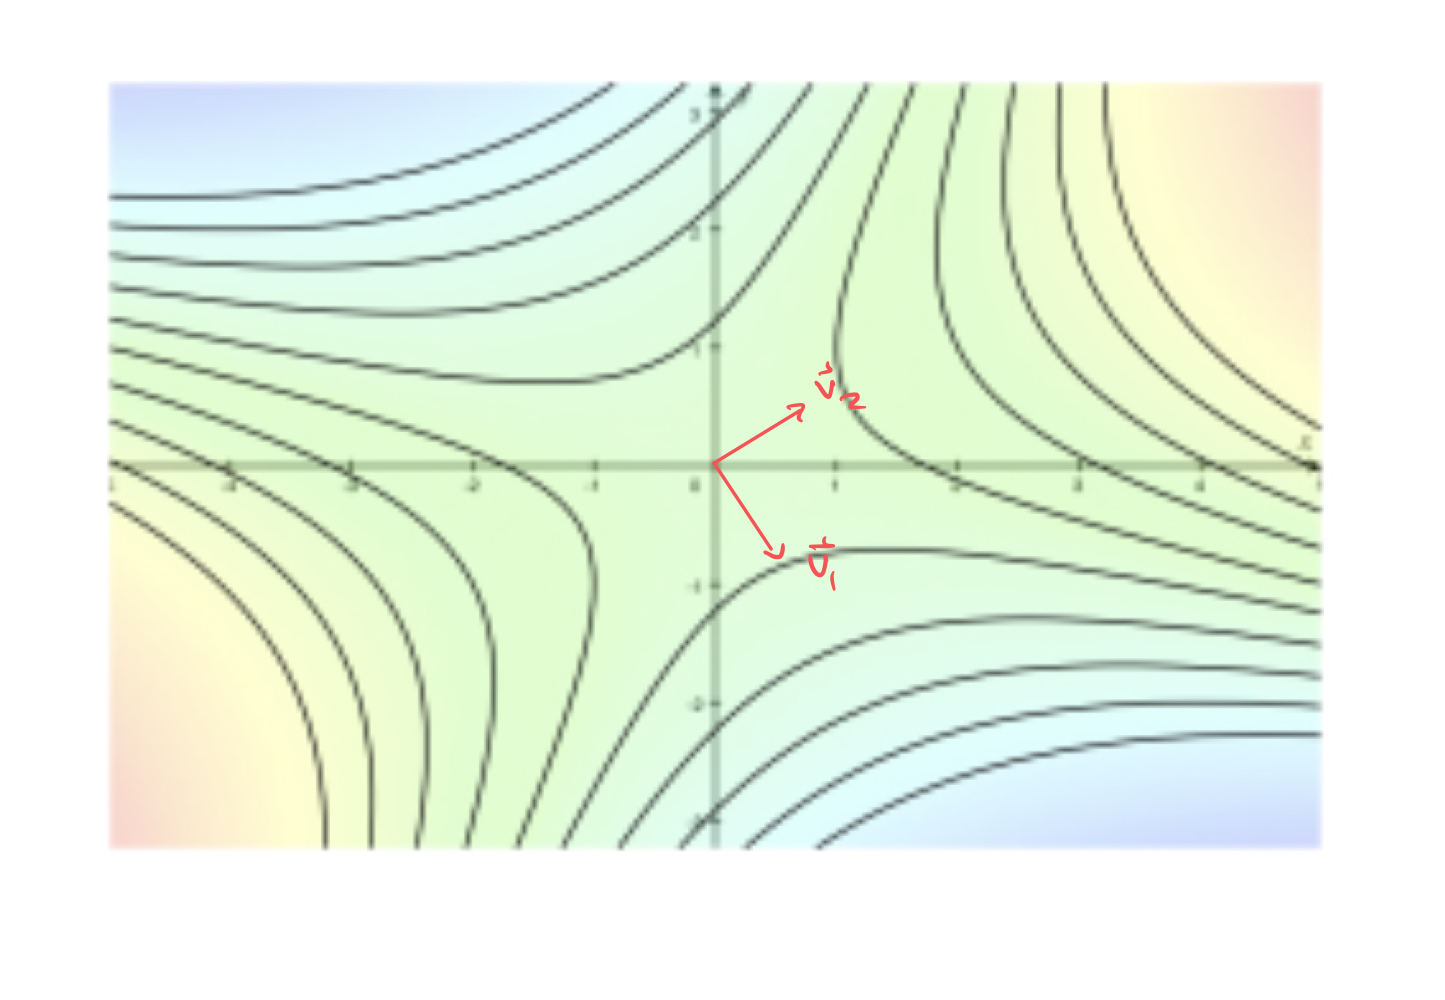
\includegraphics[scale=0.2]{contour.jpeg}
			\end{center}
			Again, as per the exam policy, I will admit that I did use Mathematica to verify my answer.
		\end{solution}
	\item Find the change of basis matrix $C$ that diagonalizes $Q_{[e]}$. What is the diagonalized matrix
		$Q_{[f]}$? Show that in the eigenbasis, Eq. 5 decouples and find the ODE for the variable $c_1$. 
		Use the change-of-basis matrix to find the components $\vec r_{[f]}$ for the position vector 
		$\vec r_{[e]} = \begin{pmatrix} 1\\2 \end{pmatrix} $.

		\begin{solution}
			The matrix that will diagonalize $Q_{[e]}$ is going to be composed of the eigenvectors of $Q$, so
			\[
				C = \begin{pmatrix} \sqrt{3}/2 & 1 / 2\\ 1 / 2& -\sqrt{3} /2  \end{pmatrix} = \frac{1}{2}
				\begin{pmatrix} \sqrt{3} & 1\\ 1 & -\sqrt{3}  \end{pmatrix} 
			\] %check this later 
			Furthermore, we know that the diagonalized form of the matrix $Q_{[f]}$ is going to be a diagonal
			matrix with eigenvalues on the diagonal:
			\[
				Q_{[f]} = \begin{pmatrix}  \gamma & 0 \\ 0 & 5 \gamma  \end{pmatrix} 
			\] 
			In the eigenbasis, the differential matrix equation still holds:
			\[
				\ddot {\vec r}_{[f]} = -\frac{1}{m} Q_{[f]} \vec r_{[f]} = -\frac{1}{m}\begin{pmatrix} \gamma & 0 \\ 0 & 5 \gamma \end{pmatrix} \begin{pmatrix} c_1 \\ c_2 \end{pmatrix} = -\begin{pmatrix} \frac{\gamma}{m} c_1 \\ \frac{5\gamma}{m} c_2 \end{pmatrix} 
			\] 
			This gives us two independent differential equations:
		\begin{align*}
			\ddot c_1(t) = -\frac{\gamma}{m}c_1\\
			\ddot c_2(t) = -\frac{5\gamma}{m}c_2
		\end{align*}
		hence they are decoupled. Finally, to find $\vec r_{[f]}$ for $\vec r_{[e]} = 
		\begin{pmatrix} 1\\2 \end{pmatrix} $, we use the relation $\vec r_{[f]} = C^{-1} \vec r_{[e]}$. First, 
		we notice that the set $\{\hat{f}_i\}$ is actually an orthonormal set:
		\[
			\hat{f}_1 \cdot \hat{f}_2 = \frac{1}{2}\left( \sqrt{3} - \sqrt{3}  \right) = 0
		\] 
		and we know that the set $\{\hat{e}_i\}$ is also orthonormal. Since both sets are orthonormal, 
		then we have the result from lecture that $C$ (the change of basis matrix) must be unitary. Therefore, 
		$C^{-1} = C^\dagger$:
		\[
			C^{-1} = C^{\dagger} = \frac{1}{2}\begin{pmatrix} \sqrt{3}  & 1 \\ 1 & -\sqrt{3}  \end{pmatrix} 
		\] 
		(As per the exam policy, I admit that I did use Mathematica to check that this is indeed the inverse.) 
		Therefore, we can now calculate $\vec r_{[f]}$:
		\[
			\vec r_{[f]} = \frac{1}{2}\begin{pmatrix} \sqrt{3} & 1 \\ 1 & -\sqrt{3}  \end{pmatrix} \begin{pmatrix} 1\\2 \end{pmatrix} = \frac{1}{2}\begin{pmatrix} \sqrt{3} +2\\ 1 - 2\sqrt{3}  \end{pmatrix} 
		\] 
		\end{solution}
	\item Find all possible values of $w_1$ and $w_2$ in terms of $\gamma$ such that $\vec r_1(t) = 
		e^{i w_1 t} \hat{f}_1$ and $\vec r_2(t) = e^{i w_2 t} \hat{f}_2$ solve Eq. 5. From this, determine
		the most general real solution $r(t)$ in terms of $\hat{f}_i$ and $\gamma$. Finally, briefly describe
		how to find $\vec r_{[e]}(t)$ given initial conditions $\vec r_{[e]}(0)$ and $\vec v_{[e]}(0) = 
		\dot{\vec r}_{[e]}(0)$. 
		
		\begin{solution}
			The most general real solution $\vec r(t)$ is composed of a linear combination of these two 
			vectors $\vec r_1(t)$ and $\vec r_2(t)$:
			\[
			\vec r(t) = \begin{pmatrix} r_1(t) \\ r_2(t) \end{pmatrix} 
			\] 
			From the earlier decoupling, we know that $\vec r_1(t)$ and $\vec r_2(t)$ are a part of two 
			independent differential equations, since the eigenbasis decouples these two equations:
			\begin{align*}
				\ddot r_1(t) &= -\frac{\gamma}{m}r_1(t) \\
				\ddot r_2(t) &= -\frac{5\gamma}{m}r_2(t)
			\end{align*}
			Letting $r_1(t) = e^{i w_1 t}$ (we neglect the $\hat{f}_1$ since it's our basis vector, and 
			here I'm only looking at the magnitude), we find:
			\[
				-w_1e^{i w_1t} = -\frac{\gamma}{m}e^{i w_1t} \implies w_1^2 = \frac{\gamma}{m} \implies 
				w_1 = \pm \sqrt{\frac{\gamma}{m}} 
			\] 
			Similarly for $r_2(t)$:
			\[
				-w_2^2 e^{i w_2t} = -\frac{5\gamma}{m}e^{iw_2t} \implies w_2^2 = \frac{5\gamma}{m} \implies
				w_2 = \pm \sqrt{5 \frac{\gamma}{m}} 
			\] 
			Now, since both differential equations are homogeneous and there are two solutions for $w_1$ and 
			$w_2$, the most general solution for $r_1(t)$ is a linear combination of the two, and the most 
			general solution for $r_2(t)$ would also be the same. Thus, the general solution for $r(t)$ is 
			the combination of these two:
			\[
			\vec r(t) = \begin{pmatrix} r_1(t) \\ r_2(t) \end{pmatrix} = \begin{pmatrix} 
		Ae^{i \sqrt{\frac{\gamma}{m}} t} + Be^{-i \sqrt{\frac{\gamma}{m}} t} \\
	Ce^{i\sqrt{\frac{5\gamma}{m}} t} + De^{-i\sqrt{\frac{5\gamma}{m}} t}\end{pmatrix} 
			\] 
			where $A, B, C, D$ represent the constants for the linear combinations. Written out in terms of 
			$\hat{f}_i$, this is:
			\[
				r_{[f]}(t) = \left( Ae^{i \sqrt{\frac{\gamma}{m}} t} + Be^{-i\sqrt{\frac{\gamma}{m}}t }\right)
				\hat{f}_1 + \left( Ce^{i \sqrt{\frac{5\gamma}{m}} t} + D e^{-i \sqrt{\frac{5\gamma}{m}} t}\right)
				\hat{f}_2
			\] 
			We can solve for $A, B, C, D$ using initial conditions. In order to find $\vec r_{[e]}(t)$, 
			there are a couple ways we can do this. Since we have the solution $\vec r_{[f]}(t)$, we can 
			transform $\vec r_{[f]}(t) \to \vec r_{[e]}(t)$ via the change of basis matrix, this time using 
			the equation $\vec r_{[e]}(t) = C \vec r_{[f]}(t)$. Then, once we have $\vec r_{[e]}(t)$, we can 
			solve for the constants $A, B, C, D$ using the given initial conditions. For each of 
			$\hat{f}_1$ and $\hat{f}_2$, there are two equations for the initial condition, meaning that 
			there are sufficiently many initial conditions to solve for the four unknowns $A, B, C, D$.
		\end{solution}
	\end{enumerate}
	\pagebreak
	\section*{Problem 3}
	\begin{enumerate}[label=\alph*)]
		\item Given Eq. 6, what are the possibilities for the rank and type of tensor that $P$ can be? For each type 
	possibility, write one possible expression for the piezoelectric equation Eq. 6 in index notation. 
	Be sure to explicitly state which contractions is/are taking place. What units must $D$ have?

	\begin{solution}
		We know the form of $\sigma$, a type (0, 2) tensor: 
		\[
			\sigma = \sigma_{ij} \hat{e}^i \otimes \hat{e}^j
		\] 
		We also know the form of $D$, a type (3, 0) tensor:
		\[
			D = D^{ijk} \hat{e}_i \otimes \hat{e}_j \otimes \hat{e}_k
		\] 
		Therefore, the tensor product $P = D \sigma$ gives us a type (3, 2) tensor, in index notation:
		\[
			P^{ijk}_{lm} = (D^{ijk} \sigma_{lm}) \hat{e}_i \otimes \hat{e}_j \otimes \hat{e}_k \otimes \hat{e}^l 
			\otimes \hat{e}^m
		\] 
		As for the different ways 
		we could contract:
		\begin{itemize}
			\item No contractions: We can leave it as is, meaning we have 
				\[
					P^{ijk}_{lm} = (D^{ijk} \sigma_{lm}) \hat{e}_i \otimes \hat{e}_j \otimes \hat{e}_k \otimes 
					\hat{e}^l \otimes \hat{e}^m
				\] 
			\item One contraction: I'll contract $i$ and $l$, which will give us a type (2, 1) tensor:
				\[
					P^{ijk}_{im} = (D^{ijk}\sigma_{im}) \hat{e}_j \otimes \hat{e}_k \otimes \hat{e}^m
				\] 
			\item Two contractions: I'll contract $i, l$ as well as $j, m$, giving us a type (1, 0) tensor:
				\[
					P^{ijk}_{ijm} = (D^{ijk} \sigma_{ij}) \hat{e}_k
				\] 
		\end{itemize}
		There are no other possibilities, since there is no dual basis vector to contract with $\hat{e}_k$, so 
		this is a complete list. As for the units of $D$, we know that $\sigma$ has units of force/area, 
		and $P$ has units charge/area. Therefore, $D$ must have units of charge/force.
	\end{solution}
\item Explicitly show that $B^{ijk} \sigma_{jk} = 0$ (this is basically saying that the anti-symmetric part of 
	$D$ doesn't contribute to the piezoelectric equation Eq. 7). 

	\begin{solution}
		We can show this by first writing out $B^{ijk}\sigma_{jk}$
		\begin{align*}
			B^{ijk}\sigma_{jk} &= \frac{1}{2}\left( D^{ijk} - D^{ikj} \right) \sigma_{jk} \\
							   &= \frac{1}{2}D^{ijk} \sigma_{jk} - \frac{1}{2}D^{ikj}\sigma_{jk}
		\end{align*}
		Now, since $\sigma_{jk}$ is a symmetric tensor, we can flip the $k$ and $j$ on the $\sigma$ in the 
		second term without changing the expression, giving:
		\[
			\frac{1}{2}D^{ijk}\sigma_{jk} - \frac{1}{2}D^{ikj} \sigma_{kj}
		\] 
		Now notice that these are actually the exact same summation since the indices line up perfectly. To 
		be a bit more explicit, let's swap $k$ and $j$ on the second term (we can do this since they're dummy
		indices):
		\[
			B^{ijk} \sigma_{jk} = \frac{1}{2}D^{ijk} \sigma_{jk} - \frac{1}{2}D^{ijk} \sigma_{jk} = 0
		\] 
		Therefore, we conclude that $B^{ijk}\sigma_{jk} = 0$. 
	\end{solution}
\item How many independent components does $D$ have? (Note that we are in three-dimensions here!)

	\begin{solution}
		Since $D^{ijk} = D^{ikj}$, this means that there's symmetry in $j$ and $k$. Thus, for the pair $(j, k)$,
		there are six independent components: $(j, k) = (1, 1), (1, 2), (1, 3) (2, 2), (2, 3), (3, 3)$. For
		each of these, we can have $i = 1, 2, 3$ since there aren't any restrictions on $i$, so therefore 
		there are $3 \times 6 = 18$ independent components.
	\end{solution}
\item How do the components of $D^{ijk}$ and $\sigma_{jk}$ of the piezoelectric and stress tensors transform
	under $S$?

	\begin{solution}
		$S$ is an active transformation, and we know that for a general tensor, they transform as follows
		under an active transformation (from the big tensor table):
		\[
			T'^{i_1, \dots, i_p}_{j_1, \dots, j_p} = S^{i_1}_{k_1} \cdots S^{i_p}_{k_p} T^{k_1, \dots, k_p}_{l_1, \dots l_q} (S^{-1})^{l_1}_{j_1} \cdots (S^{-1})^{l_q}_{j_q}
		\] 
		Therefore, applying this property to our tensors $D$ and $\sigma$:
		\[
			D'^{ijk} = S^i_l S^j_m S^k_n D^{lmn} \ \ \sigma_{jk} = \sigma_{lm} (S^{-1})^l_j (S^{-1})^m_k
		\] 
	\end{solution}
\end{enumerate}
\end{document}
